\subsection{Rayleigh-B\'enard-Konvektion}
Rayleigh-B\'enard-Konvektion ist eine Form von Konvektion, die durch einen Dichtegradienten und Gravitation verursacht wird. 
Sie tritt zum Beispiel auf wenn eine Flüssigkeit von unten erhitzt wird, wie es in einem Kochtopf der Fall ist. 
Der Temperaturgradient führt zu Dichteunterschieden im Fluid. Durch diese und die Gravitation wird wärmeres Fluid durch die Auftriebskraft nach oben gedrückt, während kaltes Fluid aus dem selben Grund nach unten sinkt.
Oben angekommen kühlt das warme Fluid ab, und sinkt wieder nach unten. 
Das Zusammenspiel von steigendem und sinkendem Fluid führt zur Entstehung von sogenannten Konvektionswalzen (auch \emph{large scale circulations}). 
Diese Konvektionswalzen führen zu einer Durchmischung der Flüssigkeit und damit zu einer homogenen Temperatur im Inneren der Walze. Der schematische Temperaturverlauf ist in \cref{fig:scheme_t} zu sehen.
Konvektionswalzen können abhängig von Randbedingungen, wie der Form des Gefäßes indem sich das Fluid befindet, unterschiedliche Strukturen bilden wie z.B. rechteckige und hexagonale Prismen und Spiralen \cite{Structures}.
\\
Neben den Walzen der Rayleigh-B\'enard-Konvektion treten auch sogenannte \mbox{\emph{Plumes}} auf. Dabei handelt es sich um lokale Wolken, die eine von ihrer unmittelbaren Umgebung verschiedene Temperatur haben. Durch den Temperaturunterschied zur Umgebung, bewegt sich ein Plume in der Regel schneller durch das Fluid, als die Konvektionswalze sich dreht. Allerdings wird im Zuge dieses Versuchs angenommen, dass die Plumes der Konvektionswalze folgen und eine sehr ähnliche Geschwindigkeit besitzen. 

\begin{figure}
\begin{subfigure}{0.45\textwidth}
	% GNUPLOT: LaTeX picture with Postscript
\begingroup
  \makeatletter
  \providecommand\color[2][]{%
    \GenericError{(gnuplot) \space\space\space\@spaces}{%
      Package color not loaded in conjunction with
      terminal option `colourtext'%
    }{See the gnuplot documentation for explanation.%
    }{Either use 'blacktext' in gnuplot or load the package
      color.sty in LaTeX.}%
    \renewcommand\color[2][]{}%
  }%
  \providecommand\includegraphics[2][]{%
    \GenericError{(gnuplot) \space\space\space\@spaces}{%
      Package graphicx or graphics not loaded%
    }{See the gnuplot documentation for explanation.%
    }{The gnuplot epslatex terminal needs graphicx.sty or graphics.sty.}%
    \renewcommand\includegraphics[2][]{}%
  }%
  \providecommand\rotatebox[2]{#2}%
  \@ifundefined{ifGPcolor}{%
    \newif\ifGPcolor
    \GPcolortrue
  }{}%
  \@ifundefined{ifGPblacktext}{%
    \newif\ifGPblacktext
    \GPblacktexttrue
  }{}%
  % define a \g@addto@macro without @ in the name:
  \let\gplgaddtomacro\g@addto@macro
  % define empty templates for all commands taking text:
  \gdef\gplbacktext{}%
  \gdef\gplfronttext{}%
  \makeatother
  \ifGPblacktext
    % no textcolor at all
    \def\colorrgb#1{}%
    \def\colorgray#1{}%
  \else
    % gray or color?
    \ifGPcolor
      \def\colorrgb#1{\color[rgb]{#1}}%
      \def\colorgray#1{\color[gray]{#1}}%
      \expandafter\def\csname LTw\endcsname{\color{white}}%
      \expandafter\def\csname LTb\endcsname{\color{black}}%
      \expandafter\def\csname LTa\endcsname{\color{black}}%
      \expandafter\def\csname LT0\endcsname{\color[rgb]{1,0,0}}%
      \expandafter\def\csname LT1\endcsname{\color[rgb]{0,1,0}}%
      \expandafter\def\csname LT2\endcsname{\color[rgb]{0,0,1}}%
      \expandafter\def\csname LT3\endcsname{\color[rgb]{1,0,1}}%
      \expandafter\def\csname LT4\endcsname{\color[rgb]{0,1,1}}%
      \expandafter\def\csname LT5\endcsname{\color[rgb]{1,1,0}}%
      \expandafter\def\csname LT6\endcsname{\color[rgb]{0,0,0}}%
      \expandafter\def\csname LT7\endcsname{\color[rgb]{1,0.3,0}}%
      \expandafter\def\csname LT8\endcsname{\color[rgb]{0.5,0.5,0.5}}%
    \else
      % gray
      \def\colorrgb#1{\color{black}}%
      \def\colorgray#1{\color[gray]{#1}}%
      \expandafter\def\csname LTw\endcsname{\color{white}}%
      \expandafter\def\csname LTb\endcsname{\color{black}}%
      \expandafter\def\csname LTa\endcsname{\color{black}}%
      \expandafter\def\csname LT0\endcsname{\color{black}}%
      \expandafter\def\csname LT1\endcsname{\color{black}}%
      \expandafter\def\csname LT2\endcsname{\color{black}}%
      \expandafter\def\csname LT3\endcsname{\color{black}}%
      \expandafter\def\csname LT4\endcsname{\color{black}}%
      \expandafter\def\csname LT5\endcsname{\color{black}}%
      \expandafter\def\csname LT6\endcsname{\color{black}}%
      \expandafter\def\csname LT7\endcsname{\color{black}}%
      \expandafter\def\csname LT8\endcsname{\color{black}}%
    \fi
  \fi
  \setlength{\unitlength}{0.0500bp}%
  \begin{picture}(4534.00,3400.00)%
    \gplgaddtomacro\gplbacktext{%
      \csname LTb\endcsname%
      \put(176,1754){\rotatebox{-270}{\makebox(0,0){\strut{}$L$}}}%
      \put(2266,154){\makebox(0,0){\strut{}$T$}}%
    }%
    \gplgaddtomacro\gplfronttext{%
    }%
    \gplbacktext
    \put(0,0){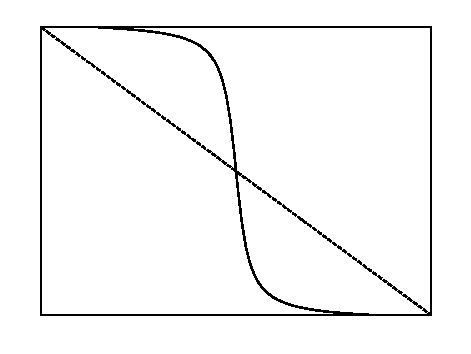
\includegraphics{temp_profile}}%
    \gplfronttext
  \end{picture}%
\endgroup
\caption{Temperaturprofil}\label{fig:scheme_t}
\end{subfigure}
\hspace{1cm}
\begin{subfigure}{0.45\textwidth}
	% GNUPLOT: LaTeX picture with Postscript
\begingroup
  \makeatletter
  \providecommand\color[2][]{%
    \GenericError{(gnuplot) \space\space\space\@spaces}{%
      Package color not loaded in conjunction with
      terminal option `colourtext'%
    }{See the gnuplot documentation for explanation.%
    }{Either use 'blacktext' in gnuplot or load the package
      color.sty in LaTeX.}%
    \renewcommand\color[2][]{}%
  }%
  \providecommand\includegraphics[2][]{%
    \GenericError{(gnuplot) \space\space\space\@spaces}{%
      Package graphicx or graphics not loaded%
    }{See the gnuplot documentation for explanation.%
    }{The gnuplot epslatex terminal needs graphicx.sty or graphics.sty.}%
    \renewcommand\includegraphics[2][]{}%
  }%
  \providecommand\rotatebox[2]{#2}%
  \@ifundefined{ifGPcolor}{%
    \newif\ifGPcolor
    \GPcolortrue
  }{}%
  \@ifundefined{ifGPblacktext}{%
    \newif\ifGPblacktext
    \GPblacktexttrue
  }{}%
  % define a \g@addto@macro without @ in the name:
  \let\gplgaddtomacro\g@addto@macro
  % define empty templates for all commands taking text:
  \gdef\gplbacktext{}%
  \gdef\gplfronttext{}%
  \makeatother
  \ifGPblacktext
    % no textcolor at all
    \def\colorrgb#1{}%
    \def\colorgray#1{}%
  \else
    % gray or color?
    \ifGPcolor
      \def\colorrgb#1{\color[rgb]{#1}}%
      \def\colorgray#1{\color[gray]{#1}}%
      \expandafter\def\csname LTw\endcsname{\color{white}}%
      \expandafter\def\csname LTb\endcsname{\color{black}}%
      \expandafter\def\csname LTa\endcsname{\color{black}}%
      \expandafter\def\csname LT0\endcsname{\color[rgb]{1,0,0}}%
      \expandafter\def\csname LT1\endcsname{\color[rgb]{0,1,0}}%
      \expandafter\def\csname LT2\endcsname{\color[rgb]{0,0,1}}%
      \expandafter\def\csname LT3\endcsname{\color[rgb]{1,0,1}}%
      \expandafter\def\csname LT4\endcsname{\color[rgb]{0,1,1}}%
      \expandafter\def\csname LT5\endcsname{\color[rgb]{1,1,0}}%
      \expandafter\def\csname LT6\endcsname{\color[rgb]{0,0,0}}%
      \expandafter\def\csname LT7\endcsname{\color[rgb]{1,0.3,0}}%
      \expandafter\def\csname LT8\endcsname{\color[rgb]{0.5,0.5,0.5}}%
    \else
      % gray
      \def\colorrgb#1{\color{black}}%
      \def\colorgray#1{\color[gray]{#1}}%
      \expandafter\def\csname LTw\endcsname{\color{white}}%
      \expandafter\def\csname LTb\endcsname{\color{black}}%
      \expandafter\def\csname LTa\endcsname{\color{black}}%
      \expandafter\def\csname LT0\endcsname{\color{black}}%
      \expandafter\def\csname LT1\endcsname{\color{black}}%
      \expandafter\def\csname LT2\endcsname{\color{black}}%
      \expandafter\def\csname LT3\endcsname{\color{black}}%
      \expandafter\def\csname LT4\endcsname{\color{black}}%
      \expandafter\def\csname LT5\endcsname{\color{black}}%
      \expandafter\def\csname LT6\endcsname{\color{black}}%
      \expandafter\def\csname LT7\endcsname{\color{black}}%
      \expandafter\def\csname LT8\endcsname{\color{black}}%
    \fi
  \fi
  \setlength{\unitlength}{0.0500bp}%
  \begin{picture}(4534.00,3400.00)%
    \gplgaddtomacro\gplbacktext{%
      \csname LTb\endcsname%
      \put(176,1754){\rotatebox{-270}{\makebox(0,0){\strut{}$v$}}}%
      \put(2266,154){\makebox(0,0){\strut{}$L$}}%
    }%
    \gplgaddtomacro\gplfronttext{%
    }%
    \gplbacktext
    \put(0,0){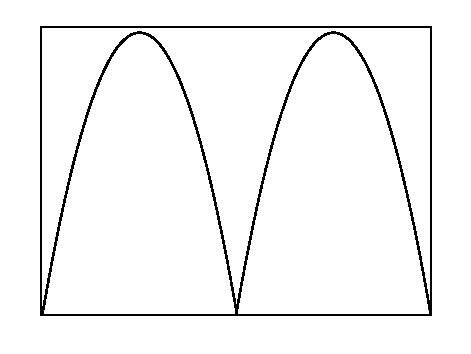
\includegraphics{vel_profile}}%
    \gplfronttext
  \end{picture}%
\endgroup
\caption{Geschwindigkeitsprofil}\label{fig:scheme_v}
\end{subfigure}
\caption{ In (\subref{fig:scheme_t}) beschreibt die durchgezogene Kurve das Temperaturprofil bei konvektivem Wärmetransport, i.e. in einer Konvektionswalze. Die gestrichelte Linie entspricht dem Temperaturprofil bei ausschließlich diffusivem Wärmetransport. (\subref{fig:scheme_v}) zeigt das Geschwindigkeitsprofil entlang einer Achse durch das Zentrum der Konvektionswalze.}
\end{figure}

\subsection{Fluidmechanik und Wärmetransport}
Grundlage für die theroretische Beschreibung der Rayleigh-B\'enard-Konvektion ist die Navier-Stokes-Gleichung. Sie beschreibt das Geschwindigkeitsfeld $\VE v$ eines Fluides unter der Wirkung von Druck-, Reibungs- und -unter Umständen- externer Kraft.
Für die Rayleigh-B\'enard-Konvektion wird die Navier-Stokes-Gleichung durch die Boussinesq-Näherung vereinfacht \cite{tritton}.
Diese Näherung besteht in der Annahme, dass die Dichte $\rho$ des Fluides nicht vom Druck $p$ abhängt, sondern lediglich linear mit der Temperatur $T$ verbunden ist über die \cref{eq:bouss}:
\begin{align}
\rho-\rho_0 = -\rho_0\alpha(T-T_0). \label{eq:bouss}
\end{align}
Hierbei ist $\rho_0$ die Dichte der Flüssigkeit bei einer Referenztemperatur $T_0$. Der Koeffizient $\alpha$ bezeichnet den thermischen Ausdehungskoeffizienten. Zudem wird angenommen, dass alle anderen physikalischen Größen unabhängig von der Temperatur sind.
\\
Mit dieser Näherung ergibt sich die Navier-Stokes-Gleichung zu \cref{eq:navier} \cite{Structures}:
\begin{align}
\frac{1}{\text{Pr}}\left(\frac{\partial}{\partial t} \VE v + \VE v \cdot \nabla \VE v \right) -\Delta \VE v + \nabla p = \text{Ra} \VE e_z \label{eq:navier}
\end{align}
Hierbei ist die Gleichung in eine dimensionslose Form gebracht worden. 
Neben der Navier-Stokes-Gleichung spielen die Kontinuitätsgleichung und die Wärmetransportgleichung eine Rolle für die Realisierung der Rayleigh-B\'enard-Konvektion in diesem Versuch. 
Die beiden dimensionslosen Kennzahlen in \cref{eq:navier} bezeichnen die Rayleigh- und die Prandtl-Zahl, die sich jeweils als 
\begin{align}
	\text{Ra} &= \frac{g\alpha\Delta T L^3}{\kappa\nu} \label{eq:rayleigh}, \\
	\text{Pr} &= \frac{\nu}{\kappa} \label{eq:prandtl}
\end{align}
ergeben \cite{Structures}. Mit Erdbeschleunigung $g$, Temperaturunterschied $\Delta T = T-T_0$, charakteristischer Länge $L$, thermischer Diffusivität $\kappa$ und kinematischer Viskosität $\nu$.
\\
Wie man bereits aus \cref{eq:prandtl} entnehmen kann, beschreibt die Prandtl-Zahl das Verhältnis von Viskosität zu Diffusivität. Die Rayleigh-Zahl gibt Aussage darüber ob der Wärmetransport in einem Fluid diffusiv oder konvektiv erfolgt. Unterhalb einer kritischen Rayleigh-Zahl $\text{Ra}_{crit}$ findet der Wärmetransport nur durch Diffusion statt. Für diesen Versuch ergibt sich etwa ein Wert von $\text{Ra}_{crit} = 1700$ \cite{Racrit}.
Ein kurzer Überblick der Kennzahlen für Systeme, in denen Konvektion stattfindet ist in \cref{tab:rayl} zu sehen.
\\
\begin{table}[!h]
        \centering
        \begin{tabular}{l|llll}
                & Erdkern & Erdmantel & Atmosphäre &Zelle \\ \hline
                $\Ra$&   \num{1.0e31}&\num{2.3e7} &\num{2.4e22}&\num{1.1e9}           \\
                $\Pr$&   \num{2.7e-2} &\num{1.2e23}&\num{5.7e-1} &\num{7.0} 
	\end{tabular}
\caption{Typische Rayleigh- und Prandtl-Zahlen im Vergleich. Da das Innere des Erdkerns fest
ist, kann nur im äußeren Erdkern RBK stattfinden. Bei der Atmosphäre gibt es lediglich
in der Troposphäre den für RBK erforderlichen Temperaturverlauf.
Stoffkonstanten dargestellt in~\cref{ch:appendix}. }
\label{tab:rayl}
\end{table}
Wird die Konvektion durch einen Temperaturunterschied verursacht, und nicht etwa einen chemischen Gradienten, so lässt sich die Konvektion anhand einer weiteren Kennzahl klassifizieren. 
Die Nusselt-Zahl beschreibt das Verhältnis des gesamten Wärmetransports zum rein diffusiven Transport eines ruhenden Fluids \cref{eq:nus_inte}.
\begin{align}
	\text{Nu}= \frac{\text{gesamter Wärmetransport}}{\text{idealer diffusiver Transport}}. \label{eq:nus_inte}
\end{align}
Der gesamte Wärmetransport entspricht dem Integral des Wärmestroms über die Grenzen des betrachteten Volumens. 
Für einen hauptsächlich advektiven Wärmetransport lässt sich die Nusselt-Zahl auch  mit \cref{eq:nus_grenz} bestimmen.
\begin{align}
	\text{Nu} = \frac{L}{2\delta} .\label{eq:nus_grenz}
\end{align}
Hierbei bezeichnet $\delta$ die Dicke der thermischen Grenzschicht. Diese ist definiert als das Regime des diffusiven Wärmetransports in unmittelbarer Nähe des Randes der Konvektionszelle. Sie kann auch in der schematischen Darstellung aus \cref{scheme_t} erkannt werden.
Aus Messwerten lässt sich die Dicke der Grenzschicht bestimmen, indem die Temperatur im diffusiven Regime und im konvektiven Regime durch zwei lineare Funktionen genähert wird. Der Schnittpunkt der Funktion entspricht der Dicke der Grenzschicht. \label{sec:grenz}
\\
Die Haftbedingung der Fluidmechanik bedingt ein besonderes Geschwindigkeitsprofil. Die Geschwindigkeit an den Grenzen der Konvektionszelle muss verschwinden. Zugleich verschwindet die Geschwindigkeit aber auch im Zentrum der Rotation. Dadurch ergibt sich das in \cref{fig:scheme_v} zu sehende Geschwindigkeitsprofil.

